\documentclass[11pt]{article}

% find things that are incomplete: TODO

%%%%%%%%%%%%%%%%%%%%%%%%%%%%%%%%%%%%%%%%%%%%%%%%%%%%%%%%
% Imports 		%%%%%%%%%%%%%%%%%%%%%%%%%%%%%%%%%%%%%%%%
%%%%%%%%%%%%%%%%%%%%%%%%%%%%%%%%%%%%%%%%%%%%%%%%%%%%%%%%

	\usepackage{amsmath,amsfonts,amsthm,amssymb,amsopn,bm} %%% load AMS-Latex Package
	\usepackage{graphics,graphicx,subfigure,color} %figures and color	
	\usepackage{mathrsfs}

	%%% paper layout, stylistic etc
	\usepackage{epsfig,fullpage}
	\usepackage{url}
	\usepackage[pdfborder={0 0 1}, colorlinks=true, citecolor=black, plainpages=false]{hyperref}
	\usepackage{parskip} %dont indent paragraphs
	\usepackage[makeroom]{cancel}


	\usepackage{tikz} % graphical models
	\usetikzlibrary{chains,fit,shapes}
	\usetikzlibrary{bayesnet}


%%%%%%%%%%%%%%%%%%%%%%%%%%%%%%%%%%%%%%%%%%%%%%%%%%%%%%%%
% Commands 		%%%%%%%%%%%%%%%%%%%%%%%%%%%%%%%%%%%%%%%%
%%%%%%%%%%%%%%%%%%%%%%%%%%%%%%%%%%%%%%%%%%%%%%%%%%%%%%%%

	\newcommand{\vct}[1]{\boldsymbol{#1}} % vector
	\newcommand{\mat}[1]{\boldsymbol{#1}} % matrix
	\newcommand{\cst}[1]{\mathsf{#1}} % constant
	\newcommand{\T}{^{\textrm T}} % transpose

	\newcommand{\inner}[2]{#1\cdot #2}
	\newcommand{\norm}[1]{\left\|#1\right\|}
	\newcommand{\twonorm}[1]{\|#1\|_2^2}

	\newcommand{\ProbOpr}[1]{\mathbb{#1}} % hollow letter
	\newcommand{\SetOf}[1]{\mathbf{#1}} % Capital set bold letter

	\newcommand{\degrees}[1]{#1$^{\circ}$} % degrees
	\newcommand{\prob}[1]{\text{p}(#1)} % probability

	\DeclareMathOperator*{\argmin}{argmin}
	\DeclareMathOperator*{\argmax}{argmax}

	\newcommand{\Eq}[1]{\begin{align*}#1\end{align*}} % conditional expectation

	\newcommand{\italic}[1]{\textit{#1}} % italic
	\newcommand{\boldFace}[1]{\textbf{#1}} % bold

	\newcommand{\cursive}[1]{\mathcal{#1}}
	\newcommand{\script}[1]{\mathscr{#1}}

%%%%%%%%%%%%%%%%%%%%%%%%%%%%%%%%%%%%%%%%%%%%%%%%%%%%%%%%
% Document 		%%%%%%%%%%%%%%%%%%%%%%%%%%%%%%%%%%%%%%%%
%%%%%%%%%%%%%%%%%%%%%%%%%%%%%%%%%%%%%%%%%%%%%%%%%%%%%%%%

\title{Probabilistic Graphical Models Notes}
\author{Chet Corcos}

\begin{document}

\maketitle
\tableofcontents

\newpage

\section{Probability Review}

	$\SetOf{X}$ is a random variable and $x$ is a possible varile of the random variable. $\prob{\SetOf{X}}$ is therefor a distribution and $\prob{\SetOf{X}=x} = \prob{x} \in [0,1]$ is a probability.

	\begin{itemize}
		\item joint distribution: \Eq{\prob{x,y}}
		\item marginal distribution: \Eq{\prob{x} = \sum_{y \in \SetOf{Y}} \prob{x,y}}
		\item conditional distribution: \Eq{\prob{x|y} = \frac{\prob{x,y}}{\prob{y}}}
		\item Bayes' Theorem: \Eq{\prob{x,y} &= \prob{x|y}\prob{y} \\&= \prob{y|x} \prob{x}\\ \prob{x|y} &= \frac{\prob{y|x}\prob{x}}{\prob{y}}}
		\item independence: $x \perp y$ \Eq{\prob{x|y} &= \prob{x}\\\prob{x,y} &= \prob{x}\prob{y}}
		\item conditional independence: $x \perp y | z$ \Eq{\prob{x|y,z} &= \prob{x|z}\\\prob{x,y|z} &= \prob{x|z}\prob{y|z}}
	\end{itemize}

\section{Bayesian Network (BN)}
	A Bayesian Network is a graph defined by verticies and directed edges with no cycles, also known as a directed acyclic graph (DAG).
	\Eq{\cursive{G}=(\cursive{V},\cursive{E})} 
	$\cursive{V}$: a vertex reprsents a random varaible.\\ 
	$\cursive{E}$: edge represents a dependence, correlation, causality, evidence between random variables.

	The structure of a BN encodes the independencies and conditional independencies. 

	In general, for any BN, the joint distribution can be decomposed as:

	\Eq{\prob{\SetOf{X}_1,\SetOf{X}_2,...\SetOf{X}_N}&= \prod_{i=1}^N \prob{\SetOf{X}_i|\text{parents}(\SetOf{X}_i)}}

	For example:

	\begin{center}
	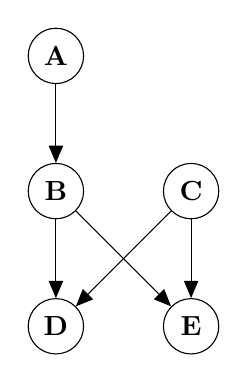
\begin{tikzpicture}
		% Define nodes
		\node[latent] (A) {$\SetOf{A}$};
		\node[latent, below=of A] (B) {$\SetOf{B}$};
		\node[latent, right=of B] (C) {$\SetOf{C}$};
		\node[latent, below=of B] (D) {$\SetOf{D}$};
		\node[latent, below=of C] (E) {$\SetOf{E}$};

		% Connect the nodes
		\edge {A} {B};
		\edge {B,C} {D,E};
	\end{tikzpicture}
	\end{center}

	\Eq{\prob{\SetOf{A},\SetOf{B},\SetOf{C},\SetOf{D},\SetOf{E}} &= \prob{\SetOf{A}}\prob{\SetOf{B}|\SetOf{A}}\prob{\SetOf{C}}\prob{\SetOf{D}|\SetOf{B},\SetOf{C}}\prob{\SetOf{E}|\SetOf{B},\SetOf{C}}}

	\begin{itemize}
		\item $\SetOf{A}$ and $\SetOf{C}$ are marginally independent (independent of all other variables).
		\item $\SetOf{B}$ is dependent on $\SetOf{A}$
		\item $\SetOf{B} \perp \SetOf{C}$
		\item $\SetOf{D} \perp \SetOf{E} | \SetOf{B}, \SetOf{C}$ but $\SetOf{D} \cancel{\perp} \SetOf{E}$
	\end{itemize}

	For discrete sets of random variables, the edges are represented as conditional probability tables. For example, if there are 2 outcomes for each random variable $\SetOf{A} = \{a_1, a_2\}$ and $\SetOf{B} = \{b_1,b_2\}$, then the relationship for $\prob{\SetOf{B}|\SetOf{A}}$ is encoded as:

	\begin{table}[h]
		\caption{Simple CPT Example}
		\centering
		\begin{tabular}{c|c c} % number of columns and vertical lines
			& $a_1$ & $a_2$\\
			\hline
			$b_1$ & 0.5 & 0.5\\
			$b_2$ & 0.25& 0.75
		\end{tabular}
	\end{table}

	Notice that the rows sum to 1 satisfying $\sum_{\SetOf{A}} \prob{\SetOf{B|\SetOf{A}}} = 1$
 
\subsection{Naive Bayes}

	Take an example of diagnosing diseases $\SetOf{D}$ from a set of $N$ symptoms $\{\SetOf{S}_1,\SetOf{S}_2,...\SetOf{S}_N\}$. To clarify,  $\SetOf{D}$ could have multiple outcomes which are different diseases $\SetOf{D} = \{d_1,d_2,...\}$. The symptoms could be binary $\SetOf{S}_i = \{1,0\}$ or a probability $\SetOf{S}_i = [0,1]$.

	\begin{center}
	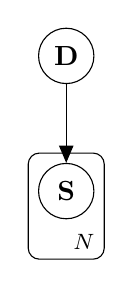
\begin{tikzpicture}
		% Define nodes
		\node[latent] (D) {$\SetOf{D}$};
		\node[latent, below=of D] (S) {$\SetOf{S}$};

		% Connect the nodes
		\edge {D} {S};
		\plate {} {(S)} {$N$}
	\end{tikzpicture}
	\end{center}


	\Eq{\prob{\SetOf{S}_1,\SetOf{S}_2,...\SetOf{S}_N,\SetOf{D}}&=\prob{\SetOf{D}}\prod_{i=1}^N \prob{\SetOf{S}_i|\SetOf{D}}}

	We can determine the probability of a disease:

	\Eq{\prob{\SetOf{D}|\SetOf{S}_1,\SetOf{S}_2,...\SetOf{S}_N}&=\frac{\prob{\SetOf{S}_1,\SetOf{S}_2,...\SetOf{S}_N,\SetOf{D}}}{\prob{\SetOf{S}_1,\SetOf{S}_2,...\SetOf{S}_N}}\\&=\frac{\prob{\SetOf{D}}\prod_{i=1}^N \prob{\SetOf{S}_i|\SetOf{D}}}{\sum_{\SetOf{D}} \prob{\SetOf{D}}\prod_{i=1}^N \prob{\SetOf{S}_i|\SetOf{D}} }}

	To determine the most likely disease:

	\Eq{\SetOf{D}^* = \argmax_{\SetOf{D}} \prob{\SetOf{D}}\prod_{i=1}^{N}\prob{\SetOf{S}_i|\SetOf{C}}}

\section{BN Semantics}
	A BN $\cursive{G} = (\cursive{V},\cursive{E})$ can be defined by the set of all independencies of the graph, $\cursive{I}(\cursive{G})$. The set of independencies can by derived from looking at each node locally or looking at every path globally.

	\subsection{Local Factorization}
	The set of all local independencies an be determined by the set of all local independencies:

	\Eq{\cursive{I}(\cursive{G}) &= \{ \cursive{V}_i \perp \text{non-decendants}(\cursive{V}_i) | \text{parents}(\cursive{V}_i) \}}

	$\text{non-decendants}(\cursive{V}_i)$ are any nodes that can by reached from following directed edged from $\cursive{V}_i$.

	\subsection{D-Separation}
	First we need to define active trail. Active trail means that there is a flow of information. Consider whether the trail between $\SetOf{X}\to \SetOf{Y}$ is active or inactive the following cases for local structures:
	\begin{itemize}
		\item Case 1

		\begin{center}
		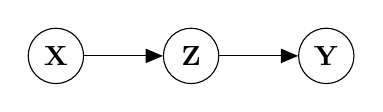
\begin{tikzpicture}
			% Define nodes
			\node[latent] (X) {$\SetOf{X}$};
			\node[latent, right=of X] (Z) {$\SetOf{Z}$};
			\node[latent, right=of Z] (Y) {$\SetOf{Y}$};
	
			% Connect the nodes
			\edge {X} {Z};
			\edge {Z} {Y};
		\end{tikzpicture}
		\end{center}
		\begin{center}
		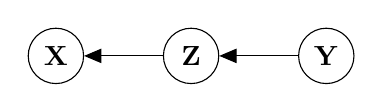
\begin{tikzpicture}
			% Define nodes
			\node[latent] (X) {$\SetOf{X}$};
			\node[latent, right=of X] (Z) {$\SetOf{Z}$};
			\node[latent, right=of Z] (Y) {$\SetOf{Y}$};
	
			% Connect the nodes
			\edge {Z} {X};
			\edge {Y} {Z};
		\end{tikzpicture}
		\end{center}
		\begin{itemize}
			\item active if $\SetOf{Z}$ is unobserved: $\SetOf{X} \cancel{\perp} \SetOf{Y}$
			\item inactive if $\SetOf{Z}$ is observed: $\SetOf{X} \perp \SetOf{Y} | \SetOf{Z}$
		\end{itemize}

		\item Case 2
		\begin{center}
		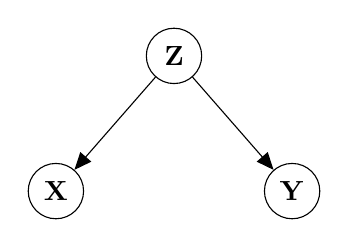
\begin{tikzpicture}
			% Define nodes
			\node[latent] (Z) {$\SetOf{Z}$};
			\node[latent, below=of Z, xshift=-1.5cm] (X) {$\SetOf{X}$};
			\node[latent, below=of Z, xshift=1.5cm] (Y) {$\SetOf{Y}$};
	
			% Connect the nodes
			\edge {Z} {Y,X};
		\end{tikzpicture}
		\end{center}

		\begin{itemize}
			\item active if $\SetOf{Z}$ is unobserved: $\SetOf{X} \cancel{\perp} \SetOf{Y}$
			\item inactive if $\SetOf{Z}$ is observed: $\SetOf{X} \perp \SetOf{Y} | \SetOf{Z}$
		\end{itemize}

		\item Case 3
		\begin{center}
		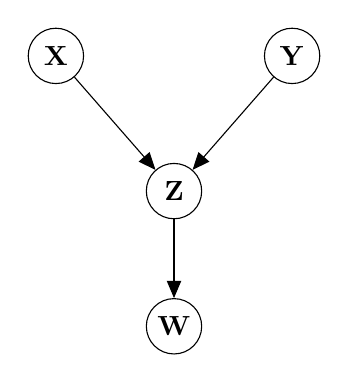
\begin{tikzpicture}
			% Define nodes
			\node[latent] (Z) {$\SetOf{Z}$};
			\node[latent, above=of Z, xshift=-1.5cm] (X) {$\SetOf{X}$};
			\node[latent, above=of Z, xshift=1.5cm] (Y) {$\SetOf{Y}$};
			\node[latent, below=of Z] (W) {$\SetOf{W}$};

			% Connect the nodes
			\edge {X,Y} {Z};
			\edge {Z} {W};
		\end{tikzpicture}
		\end{center}

		\begin{itemize}
			\item active if $\SetOf{Z}$ or any $\text{decentant}(\SetOf{Z})$ such as $\SetOf{W}$ is observed: $\SetOf{X} \cancel{\perp} \SetOf{Y}|\SetOf{Z}$ and $\SetOf{X} \cancel{\perp} \SetOf{Y}|\SetOf{W}$
			\item inactive if $\SetOf{Z}$ and all $\text{decentant}(\SetOf{Z})$ such as $\SetOf{W}$ is unobserved: $\SetOf{X}\perp \SetOf{Y}$
		\end{itemize}
	\end{itemize}

	We can no define two nodes, $\SetOf{X}$ and $\SetOf{Y}$, as being d-separated if given $\SetOf{Z}$, there is no active undirected path between them: $\text{d-sep}(\SetOf{X},\SetOf{Y}|\SetOf{Z})$. And thus, the set of all independencies of a graph can be defined as:
	\Eq{\cursive{I}(\cursive{G}) &= \{ \SetOf{X} \perp \SetOf{Y} | \SetOf{Z} : \text{d-sep}(\SetOf{X},\SetOf{Y}|\SetOf{Z}) \}}

	\subsection{I-map}

	Given a joint distribution $P$ with the set of independancies $\cursive{I}(P)$, we say that a BN graph, $\cursive{G}$, is I-map of $P$ if $\cursive{I}(\cursive{G}) \subseteq \cursive{I}(P)$. 

	% A distribution with less independence assumptions can encode all of the same information (and more) of the same distribution with more independence assummptions. Same goes for graphs. A graph $\cursive{\tilde{G}}$ formed by adding edges to $\cursive{G}$ can encode all of the same information (and more) than $\cursive{G}$. Thus $\cursive{\tilde{G}}$ is I-map of $\cursive{G}$ because $\cursive{I}(\cursive{\tilde{G}}) \subseteq \cursive{I}(\cursive{G})$. 

	A graph $\cursive{\tilde{G}}$ formed by adding edges to $\cursive{G}$ implies $\cursive{I}(\cursive{\tilde{G}}) \subseteq \cursive{I}(\cursive{G})$. Thus is $\cursive{G}$ is I-map of $P$, also $\cursive{\tilde{G}}$ is I-map of $P$.

	Note that $\cursive{I}(\cursive{G})=\emptyset$ is a valid I-map, as is the case for a fully connected graph:
	\begin{center}
	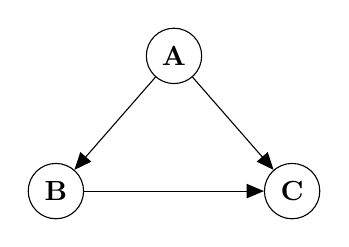
\begin{tikzpicture}
		% Define nodes
		\node[latent] (A) {$\SetOf{A}$};
		\node[latent, below=of A, xshift=-1.5cm] (B) {$\SetOf{B}$};
		\node[latent, below=of A, xshift=1.5cm] (C) {$\SetOf{C}$};
		

		% Connect the nodes
		\edge {A} {B,C};
		\edge {B} {C};
	\end{tikzpicture}
	\end{center}

	Thus $\emptyset$ is I-map of any distribution $P$. Thus, we define a \italic{minimal I-map} as an I-map such that removing any edge from a graph will result in a graph that is not I-map of the underlying distribution.

	A minimal I-map \italic{always} exists. However it is not necessarily unique. 

	\boldFace{Theorem 3.1}: (PGM Book by Koller) states that if $\cursive{G}$ is and I-map of $P$, the $P$ is factorizable to the graph.

	\boldFace{Theorem 3.2}: (PGM Book by Koller) states if $P$ factorizes according to a BN graph $\cursive{G}$, then $\cursive{G}$ is an I-map of $P$.

	These two theorems basically just say that it is valid to represent a distribution as a graph or a graph as a distribution. Any distribution can be represented by a minimal I-map graph, however, it is possible that a graph cannot encode all of the independencies of a distribution. 

	\boldFace{Theorem 3.3 (Soundness)}: (PGM Book by Koller) states that if $P$ factorized according to $\cursive{G}$, then $\cursive{I}(\cursive{G}) \subseteq \cursive{I}(P)$.

	\boldFace{Theorem 3.4 (Completeness)}: (PGM Book by Koller) states that for almost all $P$ that factorizes with respect to $\cursive{G}$, we have $\cursive{I}(\cursive{G}) = \cursive{I}(P)$.

	How these two sets of theorems differ? I'm not entirely sure. % TODO
	But it's important to note that not any set of statistical independencies can be represented by a BN. This can be proven with the gossip example.

	\subsection{Gossip Example}
	Suppose A gossips with B, B gossips with C, C gossips with D, and D gossips with A. A and C don't like each other, nor to B and D. Thus the set of independencies we would like to capture are $A \perp C|B,D$ and $B \perp D | A,C$. In fact, no BN can represent these two independencies at the same time. Thus we must introduce undirected graphical models, also known as Markov Random Fields (MRF).

\section{Markov Random Fields (MRF)}
	Markov Random Fields are represented by an undirected graph $\cursive{H} = (\cursive{V},\Phi)$ as a set of verticies and factors. A factor represents a compatibility score between two or more verticies. A factor must be positive and can be thought of as an unnormalized probability. 

	\Eq{\phi(D) \in \ProbOpr{R}^+ : D \subseteq \cursive{V}}

	The joint distribution (called a Gibbs distribution) is the product of all factors normalized by a partition function, $Z$.

	\Eq{\prob{\cursive{V}} &= \frac{1}{Z}\phi_1(D_1)\phi_2(D_2)...\phi_k(D_k)\\Z&=\sum_{\cursive{V}}\phi_1(D_1)\phi_2(D_2)...\phi_k(D_k)}


	\subsection{Gossip Example, continued}

	\begin{center}
	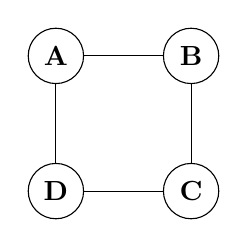
\begin{tikzpicture}
		% Define nodes
		\node[latent] (A) {$\SetOf{A}$};
		\node[latent, right=of A] (B) {$\SetOf{B}$};
		\node[latent, below=of B] (C) {$\SetOf{C}$};
		\node[latent, below=of A] (D) {$\SetOf{D}$};
		
		% Connect the nodes
		\edge [-] {A} {B,D};
		\edge [-] {C} {B,D};
	\end{tikzpicture}
	\end{center}

	The factors are defined by $D_1 = (A,B), D_2 = (B,C), D_3 = (C,D), D_4 = (D,A)$ such that:
	\Eq{\prob{A,B,C,D} &= \frac{1}{Z}\phi_1(A,B)\phi_2(B,C)\phi_2(C,D)\phi_2(D,A)\\Z&=\sum_{A,B,C,D}\phi_1(A,B)\phi_2(B,C)\phi_2(C,D)\phi_2(D,A)}

	\subsection{Graph Factorization}

	A distribution $P_\Phi$ with $\Phi = \{\phi_1(D_1)\phi_2(D_2)...\phi_k(D_k) \}$ factorizes over an undirected graph $\cursive{H}$ if $\forall\;k$, $D_k$ is a complete subgraph (commonly referred to as a clique) of $\cursive{H}$.

	For example, the following distributions all factorize over the graph:

	\begin{center}
	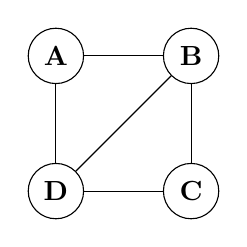
\begin{tikzpicture}
		% Define nodes
		\node[latent] (A) {$\SetOf{A}$};
		\node[latent, right=of A] (B) {$\SetOf{B}$};
		\node[latent, below=of B] (C) {$\SetOf{C}$};
		\node[latent, below=of A] (D) {$\SetOf{D}$};
		
		% Connect the nodes
		\edge [-] {A} {B,D};
		\edge [-] {C} {B,D};
		\edge [-] {D} {B};
	\end{tikzpicture}
	\end{center}

	\begin{itemize}
		\item $P_\Phi = \frac{1}{Z}\phi_1(A)\phi_2(B,C,D)$ % TODO
		\item $P_\Phi = \frac{1}{Z}\phi_1(A,D,B)\phi_2(B,C,D)$
		\item $P_\Phi = \frac{1}{Z}\phi_1(A,B)\phi_2(B,D)\phi_3(C,D)\phi_4(D,A)\phi_5(B,C)$
	\end{itemize}

	\subsection{Reduced MRF}
	Suppose we have observed some of the verticies. Given the distribution $P_\Phi(\cursive{V})$, if we observe $U=u \in \cursive{V}$ the reduced Gibbs Distribution $P_{\Phi[u]}(\cursive{V})$ is given by:
	\Eq{P_\Phi=P_\Phi(\cursive{V}) &=\frac{1}{Z}\prod_{k=1}^{K}\phi_k(D_k)\\P_{\Phi[u]}=P_{\Phi}(\cursive{V}\backslash U|U=u)&=\frac{1}{Z}\prod_{k=1}^{K}\phi_k[u](D_k\backslash U)}
	(note that the partition function $Z$ changed).

	The reduced graph, $\cursive{H}[u]$ will have fewer edges than the unreduced graph $\cursive{H}$ -- no edges are added.

	The reduced graph theorem states that $P_{\Phi}(\cursive{V}\backslash U|U=u)$ factorizes over $\cursive{H}[u]$

	\subsection{Factor Graphs}
	Consider the following undirected graph:

	\begin{center}
	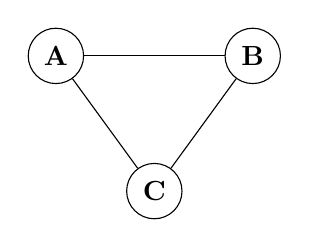
\begin{tikzpicture}
		% Define nodes
		\node[latent] (A) {$\SetOf{A}$};
		\node[latent, xshift=2.5cm] (B) {$\SetOf{B}$};
		\node[latent, below=of A, xshift=1.25cm] (C) {$\SetOf{C}$};
		
		% Connect the nodes
		\edge [-] {A} {B,C};
		\edge [-] {C} {B};
	\end{tikzpicture}
	\end{center}

	This can be represented by two different Gibbs distributions:

	\Eq{P^1_\Phi(A,B,C)&= \frac{1}{Z}\phi(A,B,C)\\P^2_\Phi(A,B,C)&= \frac{1}{Z}\phi_1(A,B)\phi_2(B,C)\phi_3(C,A)}

	However, these represent two different factor graphs:


	\begin{itemize}
		\item $P^1_\Phi(A,B,C)= \frac{1}{Z}\phi(A,B,C)$:


	\begin{center}
	\begin{tikzpicture}
		% Define nodes
		\node[latent] (A) {$\SetOf{A}$};
		\node[latent, xshift=5cm] (B) {$\SetOf{B}$};
		\node[latent, yshift=-5cm, xshift=2.5cm] (C) {$\SetOf{C}$};
		\node[factor, yshift=-2.5cm, xshift=2.5cm] (ABC) {$\phi$};

		% Connect the nodes
		\edge [-] {ABC} {A,B,C};
	\end{tikzpicture}
	\end{center}

	
		\item $P^2_\Phi(A,B,C)= \frac{1}{Z}\phi_1(A,B)\phi_2(B,C)\phi_3(C,A)$:
	
	\begin{center}
	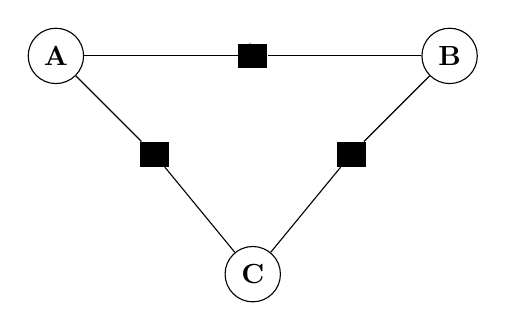
\begin{tikzpicture}
		% Define nodes
		\node[latent] (A) {$\SetOf{A}$};
		\node[factor, xshift=2.5cm] (AB) {$\phi_1$};
		\node[latent, xshift=5cm] (B) {$\SetOf{B}$};
		\node[factor, yshift=-1.25cm, xshift=3.75cm] (BC) {$\phi_2$};
		\node[factor, yshift=-1.25cm, xshift=1.25cm] (CA) {$\phi_3$};
		\node[latent, below=of CA, xshift=1.25cm] (C) {$\SetOf{C}$};

		% Connect the nodes
		\edge [-] {A} {AB,CA};
		\edge [-] {B} {AB,BC};
		\edge [-] {C} {BC,CA};
	\end{tikzpicture}
	\end{center}

	\end{itemize}

	These actually represent different distributions. A more concrete example:


	\begin{itemize}
		\item $X_1,X_2,X_3$ are independent conditioned on $Y$.

	\begin{center}
	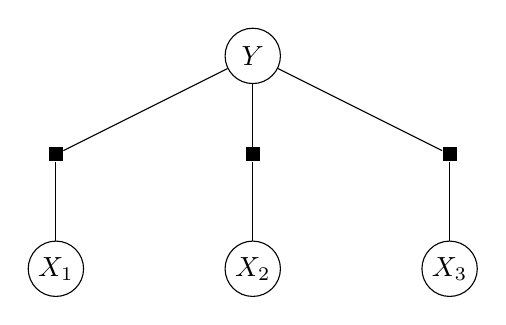
\begin{tikzpicture}
		% Define nodes
		\node[latent] (Y) {$Y$};
		\node[factor, yshift=-1.25cm,xshift=-2.5cm] (F1) {};
		\node[factor, yshift=-1.25cm,] (F2) {};
		\node[factor, yshift=-1.25cm,xshift=2.5cm] (F3){};
		\node[latent, below=of F1] (X1) {$X_1$};
		\node[latent, below=of F2] (X2) {$X_2$};
		\node[latent, below=of F3] (X3) {$X_3$};

		% Connect the nodes
		\edge [-] {F1} {Y,X1};
		\edge [-] {F2} {Y,X2};
		\edge [-] {F3} {Y,X3};
	\end{tikzpicture}
	\end{center}

	
		\item $X_1,X_2,X_3$ are NOT independent conditioned on $Y$.
	
	\begin{center}
	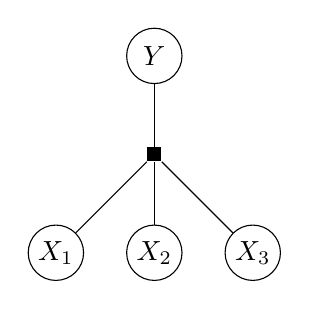
\begin{tikzpicture}
		% Define nodes
		\node[latent] (Y) {$Y$};
		\node[factor, yshift=-1.25cm] (F1) {};
		\node[latent, yshift=-2.5cm, xshift=-1.25cm] (X1) {$X_1$};
		\node[latent, yshift=-2.5cm] (X2) {$X_2$};
		\node[latent, yshift=-2.5cm, xshift=1.25cm] (X3) {$X_3$};

		% Connect the nodes
		\edge [-] {F1} {Y,X1,X2,X3};
	\end{tikzpicture}
	\end{center}

	\end{itemize}

\section{MRF Semantics}

	\subsection{Local Factorization}
	If $X,Y \in \cursive{V}$ but are not directly connected, then:
	\Eq{X\perp Y|\; \cursive{V} \;\backslash \;\{X,Y\}}

	For example, given:

	\begin{center}
	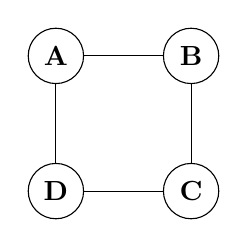
\begin{tikzpicture}
		% Define nodes
		\node[latent] (A) {$\SetOf{A}$};
		\node[latent, right=of A] (B) {$\SetOf{B}$};
		\node[latent, below=of B] (C) {$\SetOf{C}$};
		\node[latent, below=of A] (D) {$\SetOf{D}$};
		
		% Connect the nodes
		\edge [-] {A} {B,D};
		\edge [-] {C} {B,D};
	\end{tikzpicture}
	\end{center}

	\Eq{A \perp B | \; C,D}

	Applying this local factorization to all nodes, we get the Markov Blanket.

	\subsection{Markov Blanket}

	A Markov Blanket, $\text{MB}(X)$ is the set of directly connected neightbors of $X$:

	\Eq{X \perp \cursive{V} \; \backslash \; \{X,\text{MB}(X)\}|\text{MB}(X)}

	\subsection{Separation}
	We define two nodes $X$ and $Y$ as being separated with respect to $Z$ so long as $Z$ is an intermediate node for all paths $X \to Y$. 
	
	\subsection{I-map}
	Given an undirected graph, $\cursive{H}$:
	\Eq{\cursive{I}(\cursive{H}) &= \{ \SetOf{X} \perp \SetOf{Y}|\SetOf{Z} : \text{sep}(\SetOf{X},\SetOf{Y}|\SetOf{Z}) \}}

	Once again, we have soundness and completeness:
	\begin{itemize}
		\item \boldFace{Soundness}: If $P$ factorizes with $\cursive{H}$, then $\cursive{H}$ is an I-map of $P$,  $\cursive{I}(\cursive{H}) \subseteq \cursive{I}(P)$
		\item \boldFace{Hammersley-Clifford Theorem}: If $P > 0 : \forall \; x, \prob{x}>0$ and $\cursive{H}$ is an I-map of $P$, then $P$ factorizes over $\cursive{H}$.
		\item \boldFace{Completeness}: If $\cancel{\text{sep}}(X,Y|Z)$ then $X \cancel{\perp} Y | Z$ for some distribution $P$. For almost all $P$, $\cursive{I}(P) = \cursive{I}(\cursive{H})$
	\end{itemize}



	% TODO: halfway through lecture 6
	


 	\section{Review}

 	Given some distribution, $\prob{x_1, x_2, ..., x_N}$, how to we compute inferences, $\prob{x_1|x_2}$?

 	The answer is factorization. To do aid in the process, we can create a graph such as a Bayesian Network (BN), Markov Network (MN), or a factor graph. BN are directed acyclic graphs while MN are undirected and often log-linear models (exponential family distributions) or conditional random fields (CRF).

 	This all leads to graph semantics about statistical independance. The holy grail of which is d-separation which says everything you need to know about the graph structure.

 	From here, we have exact inference techniques, approximate inference techniques, and learning. 

 	For exact inference, we learned variable elimination with dynamic programming techniques such as belief propagation on a clique tree. We also learning about tree width which is the computational complexity of solving the graph.

 	For approximate inference, we learned about sampling such as monte carlo markov chain (MCMC) sampling, most notably particle filtering and gibbs sampling. We leaned about variational method and how it was derived from KL divergence. We also learned about loopy belief propagation. 

 	For learning, we have complete data and incomplete data. Both of which involve maximum likelihood estimation (MLE). Complete data is easy and convex while incomplete data requires the expectation maximization (EM) algorithm and perhaps MCMC EM ;)

 	A huge topic we did not learn about in this course is structure learning which is much much harder.

 	There are three main methods - constraint-based, score-based and optimiation/regression-based.

 	The constraint based methods suck, but they are very interesting in how they consider causality. Some well known methods are PC and K2. The goal is to learn a minimum i-map. 

 	Score-based methods are either bayesian or non-bayesian. Bayesian approiaches high highly regularized with a prior and are widely used in biology learning which genes cause which diseases. For non-bayesian techniques, its just a simple MLE but its "bullshit" because it always overfits and is an NP-HARD problem. 


 	An interesting topic in structure learning is "compressive sensing" for sprise driven models. This basically just learns the adjacency matrix of a MN.



	

\end{document}

